\chapter{Conjuntos}

El concepto de \textit{conjunto} aparece en todos los campos de las
Matemáticas, pero, ¿qué debe entenderse por él? La \textit{Teoría de conjuntos}
fue introducida por Georg Cantor (1845-1917); desde 1869, Cantor ejerció como
profesor en la Universidad de Halle y entre 1879 y 1884 publicó una serie de
seis artículos en el \textit{Mathematische Annalen}, en los que hizo una
introducción básica a la teoría de conjuntos. En su \textit{Beiträge zur
Begründung der transfiniten Mengenlehre}, Cantor dio la siguiente definición
de conjunto:

\begin{figure}[h]
  \centering
  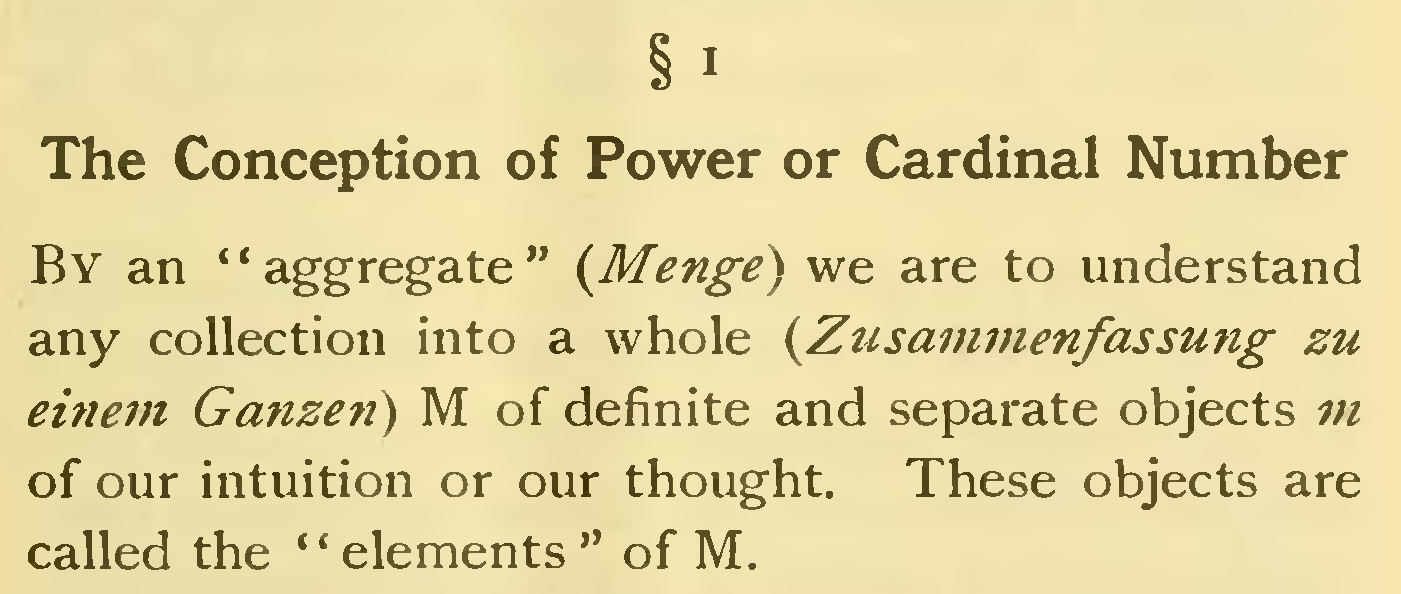
\includegraphics[scale=.2]{fig/definicionConjunto}
  \captionsetup{font=footnotesize}
  \caption{Fragmento del texto traducido al inglés en el que Cantor da la
    definición de conjunto}
\end{figure}

\begin{quote}
  <<Debemos entender por ``conjunto'' (\textit{Menge}) cualquier colección
  vista como un todo (Zusammenfassung zu einem Ganzen), $M$, de objetos
  separados y bien definidos, $m$, de nuestra intuición o pensamiento. Estos
  objetos son los ``elementos'' de $M$>>
\end{quote}

Felix Hausdorff, en 1914, dice: <<un conjunto es una reunión de cosas que
constituyen una totalidad; es decir, una nueva cosa>>, y añade: <<esto puede
difícilmente ser una definición, pero sirve como demostración expresiva del
concepto de conjunto a través de conjuntos sencillos como el conjunto de
habitantes de una ciudad o el de átomos de Hidrógeno del Sol>>.

Un conjunto así definido no tiene que estar compuesto necesariamente de
elementos homogéneos y además, da lugar a cuestiones filosóficas como si
podemos llamar \textit{conjunto} a aquel que no posee ningún elemento.
Matemáticamente, conviene aceptar solo elementos que compartan alguna propiedad
y definir el \textit{conjunto vacío} como aquel que no tiene elemento alguno.

El gran mérito de Cantor fue considerar conjuntos \textit{transfinitos} (que
tiene infinitos elementos), concepto inaudito hasta avanzado el siglo XIX,
hablar del \textit{cardinal} de un conjunto como el número de sus elementos y
hablar de \textit{conjuntos equivalentes} cuando puede establecerse una
biyección entre ellos; ideas ya apuntadas por Bolzano, quien se centró
demasiado en el aspecto filosófico, sin llegar a formalizar sus ideas.\\


A lo largo de la sección, haremos una pequeña introducción a la Teoría de
Conjuntos, presentando formalmente sus conceptos más importantes. A la hora de 
elaborar el contenido se han utilizado los siguientes recursos bibliográficos:

\begin{itemize}
\item el primer tema de la asignatura
\href{https://rodas5.us.es/file/19961ac2-66e4-4af4-bf13-81f29b771a1b/1/01-Conjuntos.pdf}
     {Álgebra Básica}\
\footnote{\url{https://rodas5.us.es/file/19961ac2-66e4-4af4-bf13-81f29b771a1b/1/01-Conjuntos.pdf}}
(\cite{Algebra-15a})

\item los temas de la asignatura 
\href{https://www.cs.us.es/~jalonso/cursos/i1m-15}
     {Informática}\
\footnote{\url{{https://www.cs.us.es/~jalonso/cursos/i1m-15}}}
(\cite{Alonso-15a}) 
 
\item el artículo de la Wikipedia
\href{https://en.wikipedia.org/wiki/Set_(mathematics)}
     {Set (mathematics)}\
\footnote{\url{https://en.wikipedia.org/wiki/Set_(mathematics)}}
(\cite{Wikipedia-grafos}) y

\item el artículo
\href{http://catedu.es/materranya/suplemento3.pdf}
     {\textit{El regalo de Cantor}}\
\footnote{http://catedu.es/materranya/suplemento3.pdf}
\end{itemize}

\section{Definiciones y propiedades}

\entrada{Conjuntos}
